\documentclass{beamer}
% preamble
\title{Exploring Anthropometric Measurements for Prediction of Body Build Weight and Gender}
\author{Damon Jia, Yi Zuo, Mindy Pike}
\institute{Vanderbilt University}
\date{May 2, 2019}

\usetheme{Boadilla}
\definecolor{VandyGold}{RGB}{212,179,125}
\usecolortheme[named=VandyGold]{structure}
\setbeamercolor*{titlelike}{fg=black,bg=VandyGold}
\setbeamercolor*{palette primary}{bg=VandyGold,fg=black}
\setbeamercolor*{palette secondary}{fg=VandyGold,bg=black}
\setbeamercolor*{palette tertiary}{bg=VandyGold,fg=black}
\setbeamercolor*{frametitle}{fg=black,bg=VandyGold}

\setbeamertemplate{footline}
{
	\leavevmode%
	\hbox{%
		\begin{beamercolorbox}[wd=.3\paperwidth,ht=2.25ex,dp=1ex,center]{author in head/foot}%
			\usebeamerfont{author in head/foot}\insertshortauthor %~~\beamer@ifempty{\insertshortinstitute}{}{(\insertshortinstitute)}
		\end{beamercolorbox}%
		\begin{beamercolorbox}[wd=.7\paperwidth,ht=2.25ex,dp=1ex,center]{title in head/foot}%
			\usebeamerfont{title in head/foot}\insertshorttitle
		\end{beamercolorbox}%
		}%
	\vskip0pt%
}

\addtobeamertemplate{navigation symbols}{}{%
	\usebeamerfont{footline}%
	\usebeamercolor[fg]{footline}%
	\hspace{1em}%
	\insertframenumber/\inserttotalframenumber
}

\begin{document}

\begin{frame}
\titlepage
\end{frame}

\begin{frame}
\frametitle{Outline}
\tableofcontents
\end{frame}

\section{Background}


\begin{frame}
\frametitle{Background}

\begin{itemize}
	\item Anthropometric measurements evaluate the size, shape, and composition of the human body
		\begin{itemize}
			\item Constant measures: skeletal measurements and three “bony” girths
		\end{itemize}
		\begin{itemize}
			\item Changeable girths: shoulder, chest, waist, navel, hip, thigh, bicep, forearm, calf
		\end{itemize}
\end{itemize}
\end{frame}

\begin{frame}

\begin{figure}
	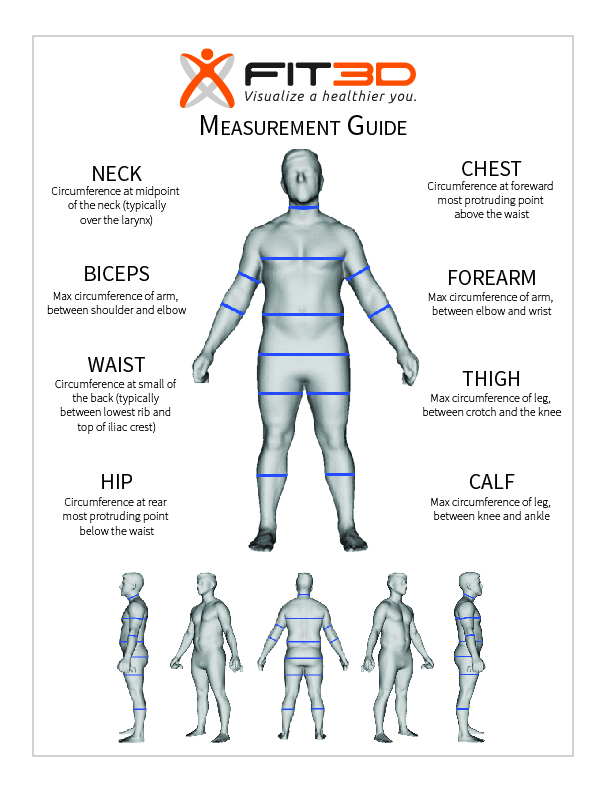
\includegraphics[scale=0.25]{Girth.jpg}
	\caption{Fit3D Male Measurement Guide}
	\label{fig:girth}
\end{figure}

\small{http://healthandfitnesstesting.nz/resources/fit3d-male-measurement-guide/}
 
\end{frame}


\section{Objective}
\begin{frame}
\frametitle{Objective}
Our objective was to evaluate the relationships between body measurements, and to develop and evaluate prediction models for body build weight and gender.

\begin{itemize}
	\item Aim 1a: Predicting weight from body build measures
	\item Aim 1b: Utility of BMI in relation to body build weight
	\item Aim 2: Predicting gender from skeletal measures
\end{itemize}

\end{frame}

\subsection{Aim 1a: Predicting weight from body build measures}

\subsection{Aim 1b: Utility of BMI in relation to body build weight}

\subsection{Aim 2: Predicting gender from skeletal measures}

\section{Methods}

\begin{frame}
\frametitle{Methods}

\begin{itemize}
	\item Description of data set:  
		\begin{itemize}
			\item 247 males and 260 females
			\item Twenties to early thirties
			\item Physically active
			\item Nine skeletal and twelve girth measurements
			\item Additional variables: height, weight, age, gender
		\end{itemize}
	\item Transformation of variables:
		\begin{itemize}
			\item Log transformation of weight
		\end{itemize}
\end{itemize}

\end{frame}

\begin{frame}
\frametitle{Aim 1a: Predicting weight from body build measures}

Linear model 
\begin{itemize}
	\item Model 1.1
		\begin{itemize}
			\item All skeletal measurements + height + gender + age
			\item Model selection: AIC criteriion
		\end{itemize}
	\item Model 1.2
		\begin{itemize}
			\item Six skeletal measurements + three constant girth measurements + height + gender +age
			\item Model selection: AIC criteriion
		\end{itemize}
\end{itemize}

\end{frame}

\begin{frame}
\frametitle{Aim 1a: Predicting weight from body build measures}

Quadratic model 
\begin{itemize}
	\item Method 1: sum, square, and multiplied by height
	\begin{itemize}
		\item Model 2.1 
			\begin{itemize}
				\item Quadratic term of all girth measures + age + gender
			\end{itemize}
		\item Model 2.2
			\begin{itemize}
				\item Quadratic term of all girth measures + age
			\end{itemize}
		\item Model 2.3
			\begin{itemize}
				\item Quadratic term of three constant girth measures + gender + age
			\end{itemize}
	\end{itemize}
	\item Method 2: multiplied by height, sum,and square
	\begin{itemize}
		\item Model 2.4
			\begin{itemize}
				\item Quadratic term of all girth measures + age + gender
			\end{itemize}
		\item Model 2.5
			\begin{itemize}
				\item Quadratic term of three constant girth measures + gender + age
			\end{itemize}
	\end{itemize}
\end{itemize}


\end{frame}


\begin{frame}
\frametitle{Aim 1b: Utility of BMI in relation to body build weight}

\begin{itemize}
	\item Body build weight
	 	\begin{itemize}
	 		\item Predicted weight from our linear model
	 		\item Normal weight given the body build frame
	 	\end{itemize}	
	\item Regressed the body build weight (log transformed) on BMI with/without gender to evaluate the utility of BMI in relation to body build weight
	\item High or low fat mass
		\begin{itemize}
			\item Difference between measured waist girth and body build waist girth predicted by chest, biiliac, and bitrochanteric diameters as well as chest depth
			\item A difference of $>$ 5 cm or $<$ -5 cm was defined as high or low fat mass
		\end{itemize}	
	\item High or low muscle mass
		\begin{itemize}
			\item Difference between measure forearm girth the body build one predicted by wrist girth, chest diameter and chest depth
			\item A difference of $>$ 1 cm or $<$ -1 cm was defined as high or low muscle mass
		\end{itemize}	
\end{itemize}

\end{frame}

\begin{frame}
\frametitle{Aim 2: Predicting gender from skeletal measures}

\begin{itemize}
	\item Logistic regression using forward and backward stepwise selection methods
	\begin{itemize}
		\item P-value for addition: 0.1
		\item P-value for removal: 0.25
	\end{itemize}
	\item Model selection completed with and without height
	\item Akaike information criterion
	\item Sensitivity and specificity
	\item Internal validation: ten-fold cross validation
	
\end{itemize}

\end{frame}

\section{Results}

\begin{frame}
\frametitle{Results}

\begin{figure}
	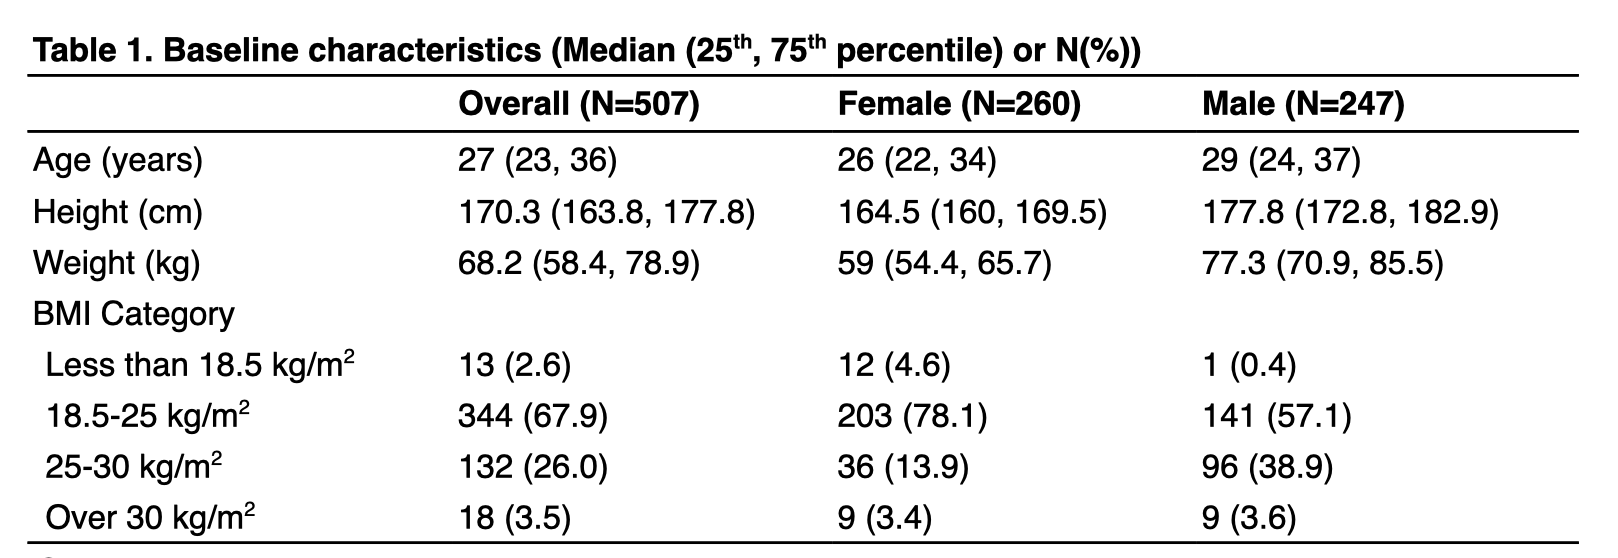
\includegraphics[scale=0.35]{Table1.png}
	\label{fig:table1}
\end{figure}

\end{frame}

\begin{frame}
\frametitle{Aim 1a: Predicting weight from body build measures}
 
\begin{itemize}
	\item Best linear model: Model 1.2
		\begin{itemize}
			\item log(weight) = skeletal biacromial + skeletal biiliac + skeletal bitrochanteric + skeletal chest depth + skeletal chest + skeletal elbow + knee girth + ankle girth + wrist girth + age + height + gender + intercept 
			\item Ten-fold cross validation yielded a pseudo $R^2$ of 0.9140.
		\end{itemize}
	\item Best quadratic model: Model 2.2
		\begin{itemize}
			\item Trasformation method 1: sum, square, and multiplied by height
			\item All girth measures in quadratic form + age
			\item Ten-fold cross validation yielded a pseudo $R^2$ of 0.9594.
		\end{itemize}
	\item Linear model was chosen due to simpler form and better interpretability.  
\end{itemize}

\end{frame}

\begin{frame}
\frametitle{Aim 1b: Utility of BMI in relation to body build weight}

\begin{itemize}
	\item Regressing body build weight on BMI
		\begin{itemize}
			\item adjusted $R^2$=0.540
			\item pseudo-$R^2$ = 0.536 by ten-fold cross-validation
 	
		\end{itemize}
	\item Regressing body build weight on BMI and gender
		\begin{itemize}
			\item adjusted $R^2$=0.748
			\item pseudo-$R^2$ = 0.750 by ten-fold cross-validation
 	
		\end{itemize}
	\item Models assessing fat mass and muscle mass
		\begin{itemize}
			\item Fat mass: adjusted $R^2$ = 0.776
			\item Muscle mass: adjusted $R^2$ = 0.787
 	
		\end{itemize}
\end{itemize}

\end{frame}

\begin{frame}
\frametitle{Aim 2: Predicting gender from skeletal measures}

Logit(gender)= chest depth + bitrochanteric + biacromial + wrist + knee + elbow + height + intercept

\begin{itemize}
	\item Forward stepwise regression 
	\item AIC: 127.0
	\item Sensitivity: 96.5\%
	\item Specificity: 95\%
	\item Internal validation $R^2$: 0.8420
\end{itemize}

\end{frame}
\begin{figure}
	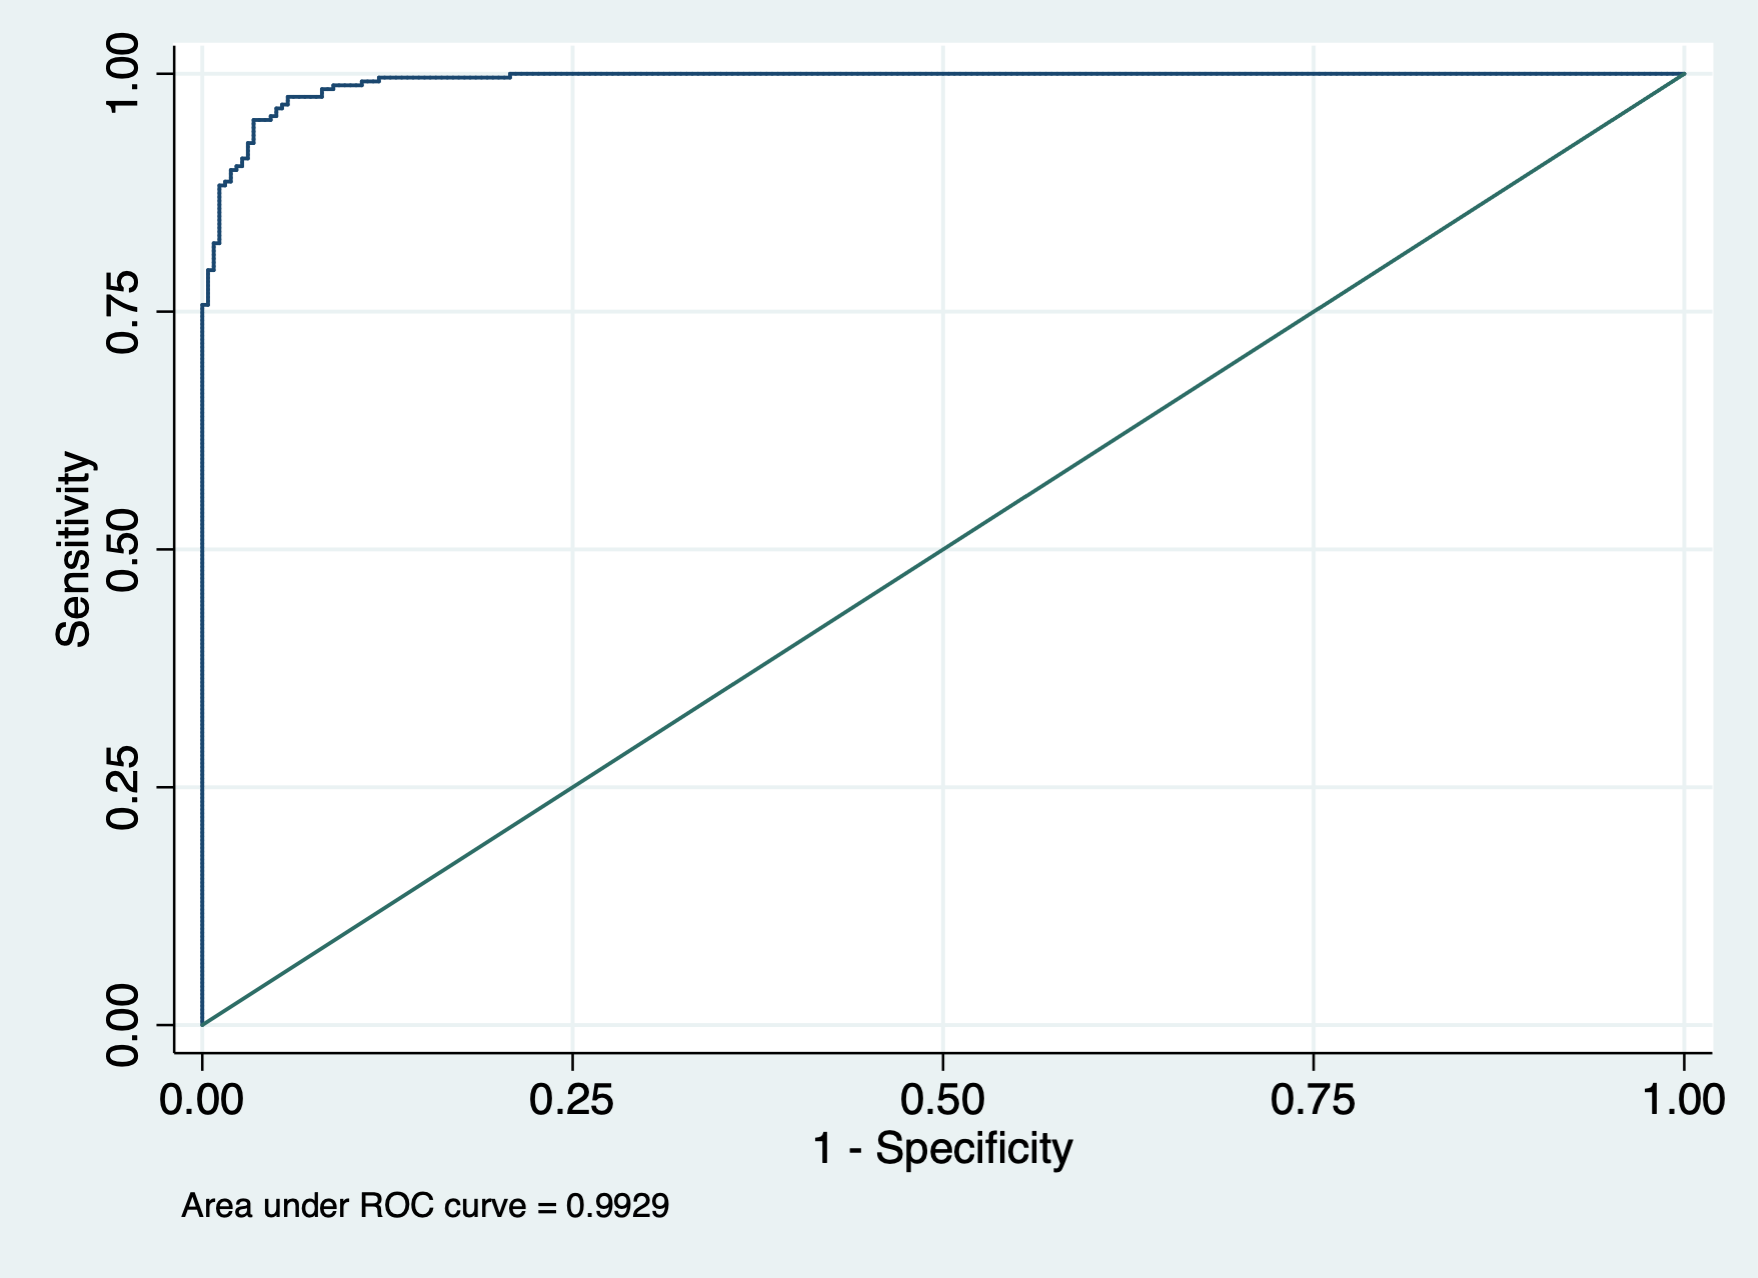
\includegraphics[scale=0.35]{Figure1.png}
	\caption{ROC curve of the prediction model}
	\label{fig:figure1}
\end{figure}

\section{Discussion}

\begin{frame}
\frametitle{Discussion}

\begin{itemize}
	\item Aim 1a
		\begin{itemize}
			\item Both linear and quadratic models show good predictability. 
			\item Linear model was chosen due to simpler form
			\item The best model contains skeletal biacromial, skeletal biiliac, skeletal bitrochanteric, skeletal chest depth, skeletal chest, skeletal elbow, knee girth, ankle girth, wrist girth, age, height, and gender. 
		\end{itemize}
	
\end{itemize}

\begin{itemize}
	\item Aim 1b
	\begin{itemize}
		\item BMI is a poor predictor for the body build weight.
		\item Subjects with high fat or muscle mass
		\begin{itemize}
			\item A larger body frame for their height
  
			\item BMI tends to classify them as overweight or obese
			\item Does not tell whether extra weight is due to fat or muscle
		\end{itemize}	
		\item Similar for subject with low fat or muscle mass
	\end{itemize}
\end{itemize}

\end{frame}

\begin{frame}
\frametitle{Discussion}

\begin{itemize}
	\item Aim 2
		\begin{itemize}
			\item Height, chest depth, bitrochanteric, biacromial, wrist, knee, and elbow skeletal measurements best predicted gender.
			\item Addition of height adds predictive ability.
		\end{itemize}
\end{itemize}

\begin{itemize}
	\item Limitations
	\begin{itemize}
		\item Different model selection methods in each aim
		\item Lack of external validation 
	\end{itemize}
\end{itemize}

\end{frame}

\begingroup
\small
\begin{frame}
\frametitle{References}
1. Heinz G, Peterson LJ, Johnson RW, Kerk CJ. Exploring Relationships in Body Dimensions. Journal of Statistics Education. 2003;11(2):null-null. doi:10.1080/10691898.2003.11910711  

2. Marks GC, Habicht J, Mueller WH. Reliability, dependability, and precision of anthropometric measurements. BioMed Research International 5 The second national health and nutrition examination survey 1976–1980. American Journal of Epidemiology. 1989:578–587.  

3. Pollock ML, Laughridge EE, Coleman B, Linnerud AC, Jackson A. Prediction of body density in young and middle-aged women. Journal of Applied Physiology. 1975;38(4):745-749. doi:10.1152/jappl.1975.38.4.745  

4. Pollock ML, Hickman T, Kendrick Z, Jackson A, Linnerud AC, Dawson G. Prediction of body density in young and middle-aged men. Journal of Applied Physiology. 1976;40(3):300-304. doi:10.1152/jappl.1976.40.3.300  

5. Wilmore JH, Behnke AR. An Anthropometric Estimation of Body Density and Lean Body Weight in Young Women. Am J Clin Nutr. 1970;23(3):267-274. doi:10.1093/ajcn/23.3.267  
\end{frame}


\begin{frame}
6. Wilmore JH, Behnke AR. An anthropometric estimation of body density and lean body weight in young men. Journal of Applied Physiology. 1969;27(1):25-31. doi:10.1152/jappl.1969.27.1.25  

7. Thorland WG, Johnson GO, Cisar CJ, Housh TJ. Estimation of Minimal Wrestling Weight Using Measures of Body Build and Body Composition. Int J Sports Med. 1987;08(6):365-370. doi:10.1055/s-2008-1025687  

8. Sebo P, Beer-Borst S, Haller DM, Bovier PA. Reliability of doctors’ anthropometric measurements to detect obesity. Preventive Medicine. 2008;47(4):389-393. doi:10.1016/j.ypmed.2008.06.012  

9. Deurenberg P, Deurenberg Yap M, Wang J, Lin FP, Schmidt G. The impact of body build on the relationship between body mass index and percent body fat. International Journal of Obesity. 1999;23(5):537-542. doi:10.1038/sj.ijo.0800868  

10. Pasco JA, Holloway KL, Dobbins AG, Kotowicz MA, Williams LJ, Brennan SL. Body mass index and measures of body fat for defining obesity and underweight: a cross-sectional, population-based study. BMC Obes. 2014;1. doi:10.1186/2052-9538-1-9  

\end{frame}

\begin{frame}
11. Romero-Corral A, Somers VK, Sierra-Johnson J, et al. Accuracy of body mass index in diagnosing obesity in the adult general population. International Journal of Obesity. 2008;32(6):959-966. doi:10.1038/ijo.2008.11  

12. Behnke, A. R., and Wilmore, J. H. (1974), Evaluation and Regulation of Body Build and Composition, Englewood Cliffs, NJ: Prentice Hall. 
 
13. Song, X., et al. "Comparison of various surrogate obesity indicators as predictors of cardiovascular mortality in four European populations." European Journal of Clinical Nutrition67.12 (2013): 1298.  

14. Joyce, C., and Stover, E. (1991), Witnesses from the Grave: The Stories Bones Tell, Boston, MA: Little, Brown, and Company, p. 80, pp. 177-178.   

15. Wingate, A. (1992), Scene of the Crime: A Writer’s Guide to Crime-Scene Investigations, Cincinnati, OH: Writer’s Digest Books, p. 148.   

\end{frame}

\begin{frame}
16. Innes, B. (2000), Bodies of Evidence: The Fascinating World of Forensic Science and How it Helped Solve More Than 100 True Crimes, Pleasantville, NY: Reader’s Digest Association, pp. 71-72.  

17. Nickell, J., and Fischer, J. F. (1999), Crime Scene: Methods of Forensic Detection, Lexington, KY: The University Press of Kentucky.  

\end{frame}
\endgroup


\begin{frame}{}
\centering \Huge
\emph{Questions?}
\end{frame}

\end{document}